\documentclass{article}
\usepackage[utf8]{inputenc}
\usepackage{amsmath}
\usepackage{float}
\usepackage{listings}
\usepackage[pdftex]{graphicx}
\usepackage{amssymb}
\usepackage{subcaption}
%--------------------------------------------------------------------

\author{Pratik Aghor}
\title{SRI Blog}
\date{\today}  % Toggle commenting to test

\begin{document}

\maketitle
%--------------------------------------------------------------------
\section*{SRI: Linear Stability}
%--------------------------------------------------------------------
%--------------------------------------------------------------------
\subsection*{Introduction}
%--------------------------------------------------------------------

We start the analysis with trying reproduce results of \cite{robins2020viscous}. The physical problem is that of stratified Taylor-Couette flow. 
TODO: Define dimensionless parameters, describe the problem, write full nonlinear-governing equations and derive the linearized equations (keep nonlinear terms till third order - for nonlinear stability later).

\begin{equation}\label{def:Re}
 Re = \frac{r_{i}\Omega_{i}d}{\nu}
\end{equation}

The base state is $(0, \Omega r, 0)$, with 
 \noindent
\begin{equation}
\Omega = A + \frac{B}{r^{2}},
\qquad
A = \frac{\mu - \eta^{2}}{1-\eta^{2}},
\qquad
B = \frac{\eta^{2}(1-\mu)}{(1+\eta)(1-\eta)^{3}},
\qquad
Z = 2A,
\label{eqn:base_state}
\end{equation}

Here $Z = (1/r) \partial_{r}(r^{2}\Omega)$ is the constant base-state vorticity. 
Centrifugal approximation $r\Omega^{2}<<g$ is made to make sure that the base state density stratification is only in the $z$ direction and the constant base-state density contours do not have curvature in the radial direction. The bouyancy frequency $N^{2} = -(g/\rho_{0})d\rho_{0}/dz$ is also assumed to be constant. This can be achieved by making the base state density $\rho_{0}$ a linear function of $z$ so $d\rho_{0}/dz$ is constant. Also, under the Boussinesq approximation, $\rho_{0}$ is assumed more or less constant, but for a weak variation in the axial direction in the bouyancy terms. The Froude number is defined as 
\begin{equation}\label{def:Fr}
 Fr = \Omega_{i}/N
\end{equation}
such that low Froude number would corrospond to strong stratification. Linear instability modes of the base state are assumed to be of the form  $\tilde{A}(r) \exp{(\sigma_{c}t + i k z + i m \theta)}$, where $\tilde{A}(r)$ is the $r$-dependent complex amplitude. 


%--------------------------------------------------------------------
\subsection*{Linearized Equations:}
%--------------------------------------------------------------------
With these assumptions the linearized equations become:
\begin{subequations}
 \begin{align}\label{eq:linearized-r-mom}
  \begin{split}
  -i\Phi u_{r} & - 2\Omega u_{\theta} \\
  &= -\frac{dP}{dr} + \frac{\eta}{(1-\eta)} \frac{1}{Re}\bigg[\frac{d^{2}u_{r}}{dr^{2}} + \frac{1}{r}\frac{du_{r}}{dr} - \bigg( \frac{m^{2} + 1}{r^{2}} + k^{2}\bigg)u_{r} - \frac{2 i m u_{\theta}}{r^{2}} \bigg],
  \end{split}
 \end{align}
 %
 \begin{align}\label{eq:linearized-theta-mom}
  \begin{split}
   -i\Phi u_{\theta} & + Z u_{r}\\
   & = \frac{-imP}{r} + \frac{\eta}{(1-\eta)} \frac{1}{Re}\bigg[\frac{d^{2}u_{\theta}}{dr^{2}} + \frac{1}{r}\frac{du_{\theta}}{dr} - \bigg( \frac{m^{2} + 1}{r^{2}} + k^{2}\bigg)u_{\theta} + \frac{2 i m u_{r}}{r^{2}}\bigg],
  \end{split}
 \end{align}
 %
 \begin{align}\label{eq:linearized-z-mom}
 -i\Phi u_{z} = -ik P - \rho  + \frac{\eta}{(1-\eta)} \frac{1}{Re}\bigg[\frac{d^{2}u_{z}}{dr^{2}} + \frac{1}{r}\frac{du_{z}}{dr}- \bigg( \frac{m^{2} + 1}{r^{2}} + k^{2}\bigg)u_{z} \bigg],
 \end{align}
 %
 \begin{align}\label{eq:linearized-rho}
  -i \Phi \rho - Fr^{-2}u_{z} = 0,
 \end{align}
 %
 \begin{align}\label{eq:linearized-continuity}
  \frac{du_{r}}{dr} + \frac{u_{r}}{r} + \frac{i m u_{\theta}}{r} + i k u_{z} = 0.
 \end{align}
\end{subequations}
Here $(u_{r}, u_{\theta}, u_{z}, \rho, P)$ are complex amplitudes of perturbations in the radial, azimutha, axial velocities and in density and pressure fields respectively. The $\Phi(r) = u\sigma_{c} - m \Omega(r) = i\sigma + \omega - m \Omega(r)$ is called the Lagrangian frequency. 

The no slip boundary conditions for the viscous flow are defined as 
\begin{equation}
 u_{r} = u_{\theta} = u_{z} = 0 
 \qquad
 \textrm{at } r = r_{i} = \frac{\eta}{1-\eta} \textrm{ and } r = r_{o} = \frac{1}{1-\eta} 
\end{equation}
%--------------------------------------------------------------------
\subsection*{Numerical Details:}
%--------------------------------------------------------------------
We adapt the standard Chebyeshev spectral method to solve the linearized system of equations, Eqns. (\ref{eq:linearized-r-mom}-\ref{eq:linearized-continuity}). Because we do not have boundary conditions for pressure-perturbation $P$ and density perturbation $\rho$, we should ideally use a staggered grid as suggested by \cite{khorrami1991chebyshev}. However, a quick look at the linearized system given by Eqns. (\ref{eq:linearized-r-mom}-\ref{eq:linearized-continuity}), we only have the $r$ derivative of the pressure perturbation, a Chebyeshev mode expansion of which will need artificial boundary conditions. Hence we only push pressure inside the domain and define it at the Gauss points given by $(x_{g})_{j} = \cos{\bigg[\frac{(2j + 1)\pi}{2N}\bigg]}$ with $j \in [0, N-1]$. We define all the other perturbation fields, namely $(u_{r}, u_{\theta}, uz, \rho)$ at the standard Gauss-Lobatto grid given by $(x_{c})_{j} = \cos{\bigg(\frac{j\pi}{2N}\bigg)}$ with $j \in [0, N]$. In this notation the subscript `$g$' stands for Gauss and the subscript `$c$' stands for the Cheyeshev-Gauss-Lobatto (or simply Gauss-Lobatto) grid. 
Both the grids are represented in the following figure on the computational domain of $[-1, 1]$:

\begin{figure}[H]
        \centering
    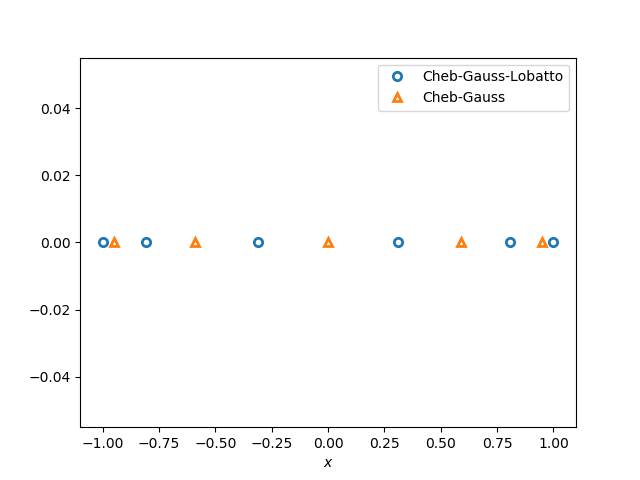
\includegraphics[scale=0.35]{Figs/test_gauss_grid.png}
            \caption{Gauss and Gauss-Lobatto grids}
        \label{fig:grids}
\end{figure}



We then need interpolation matrices to transform field quantities between Gauss- and Gauss-Lobatto-grids. As derived in \cite{khorrami1991chebyshev}, the matrices are given by the following expressions:
\begin{subequations}
 \begin{align}\label{def:G2GL}
 \begin{split}
  &[G2GL]_{jk} = \frac{(-1)^{(j + k)} (1- (x_{g})_{k}^{2})^{1/2}}{(N((x_{c})_{j} - (x_{g})_{k}))}\\
  &j \in [0, N],  k \in[0, N-1]
 \end{split}
 \end{align}
 %
 \begin{align}\label{def:GL2L}
  \begin{split}
  &[GL2L]_{jk} = \frac{(-1)^{(j + k + 1)} (1- (x_{g})_{j}^{2})^{1/2}}{(C_{k}N((x_{g})_{j} - (x_{c})_{k}))}\\
  &j \in [0, N-1],  k \in[0, N]
  \end{split}
 \end{align}
\end{subequations}

To make the matrices square, we add an extra row ($j = N$) to the $G2GL$ matrix and an extra column ($k=N$) to the $GL2G$ matrix filled with zeros. 
We obtained a good result for a test case of $y = \sin{3x}$ which are summerized in Fig. \ref{fig:test_interpolants}.
\begin{figure}[H]
\centering
\begin{subfigure}{.5\textwidth}
  \centering
  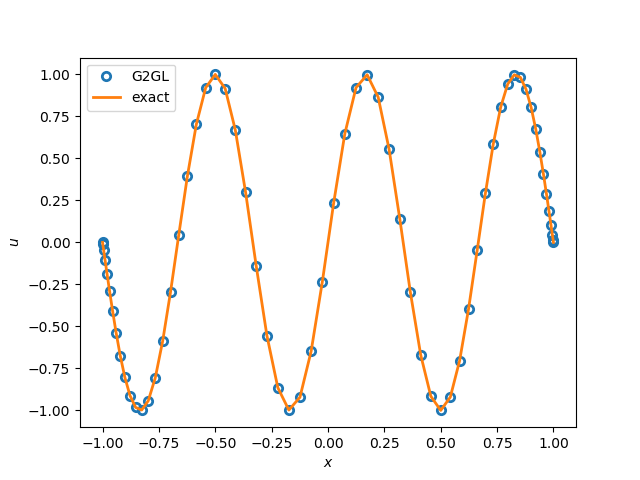
\includegraphics[scale=0.35]{Figs/test_g2gl_interpolant.png}
 \subcaption{}
  \label{fig:202a}
\end{subfigure}%
\begin{subfigure}{.5\textwidth}
  \centering
  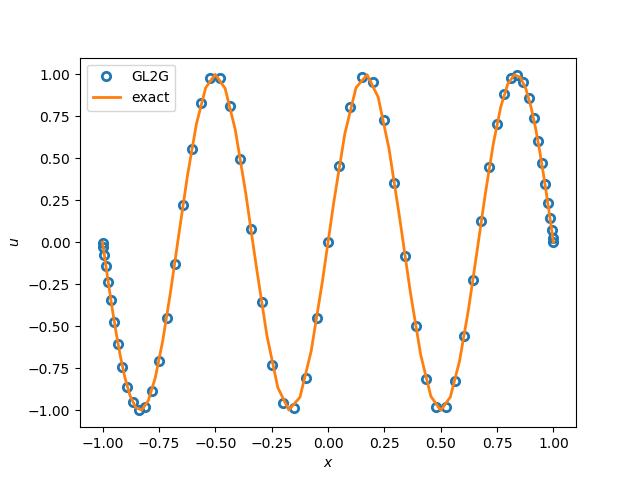
\includegraphics[scale=0.35]{Figs/test_gl2g_interpolant.png}
  \subcaption{}
  \label{fig:202b}
    \end{subfigure}
  \caption{Interpolate $\sin{3x}$ from - (a) Gauss to Gauss-Lobatto grid,  (b) Gauss-Lobatto to Gauss grid.}
\label{fig:test_interpolants}
\end{figure}

The derivatives now can be taken as, $\tilde{D}_{jk} \bigg|_{gl} = [G2GL]_{jm}D_{mk}$. where $D$ is the Chebyeshev derivative matrix. We can also explicitely find the expressions for the derivative matrices, which is advantageous because it will save an $O(N^{3})$ matrix-matrix-multiplication (henceforth matmul) process.

Assume that $P$ is known at the Gauss-grid ($j \in [0, N-1]$). To find $\frac{dP}{dx}$ at the Gauss-Lobatto grid, we write,

\begin{equation}\label{eq:dPdx_at_gl}
 \frac{dP}{dx}\bigg|_{j} = \sum_{k=0}^{N-1} E_{jk} P_{k}
\end{equation}
where the elements of $E$ are given by 
\begin{equation}
 E_{jk} = \begin{cases}
      \frac{(-1)^{(j + k + 1)} (1- (x_{g})_{k}^{2})^{1/2}}{N((x_{c})_{j} - (x_{g})_{k})^{2}}, & \text{if}\ j \in [1, N-1],   k \in [0, N-1] \\
      \frac{(-1)^{(k)} (1- (x_{g})_{k}^{2})^{1/2}}{N}\bigg( \frac{N^{2}}{1-(x_{g})_{k}} - \frac{1}{(1-(x_{g})_{k})^{2}}\bigg), & \text{if}\ j = 0,   k \in [0, N-1] \\
      \frac{(-1)^{(N+k)} (1- (x_{g})_{k}^{2})^{1/2}}{N}\bigg( \frac{N^{2}}{1+(x_{g})_{k}} - \frac{1}{(1+(x_{g})_{k})^{2}}\bigg), & \text{if}\ j = 0,   k \in [0, N-1] \\
    \end{cases}
\end{equation}
A null column ($k=N$) is added to make $E$ a square matrix. We again tested the matrix with the test function $\sin{3\pi x}$, which returned the correct derivative $3\pi\cos{3\pi x}$. 

\begin{figure}[H]
        \centering
    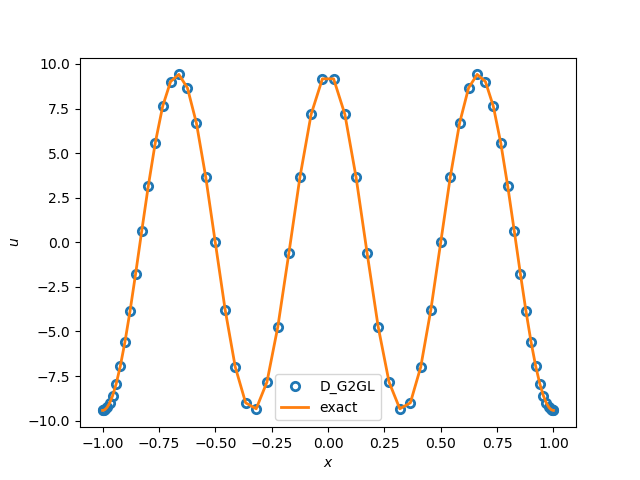
\includegraphics[scale=0.35]{Figs/test_D_g2gl_interpolant.png}
            \caption{Gauss and Gauss-Lobatto grids derivative test for $y = \sin{3\pi x}$ }
        \label{fig:test_D_g2gl_interpolant}
\end{figure}

%--------------------------------------------------------------------

%--------------------------------------------------------------------

%--------------------------------------------------------------------
%--------------------------------------------------------------------
\bibliographystyle{apalike}
%\bibliographystyle{unsrt} % Use for unsorted references  
%\bibliographystyle{plainnat} % use this to have URLs listed in References
%\cleardoublepage
%\bibliography{References/references} % Path to your References.bib file

\bibliography{bib/references} % Path to your References.bib file
 \if@openright\cleardoublepage\else\clearpage\fi
 \cleardoublepage
 \pagestyle{empty}
%--------------------------------------------------------------------
\end{document}
